\documentclass[]{article}
\usepackage[a4paper, total={15cm,23cm}]{geometry}
\usepackage{fancyhdr}
\usepackage{graphicx}
\usepackage{amsmath}
\usepackage{amssymb}
\usepackage{xcolor}
%opening
\title{PH 223 Activity 4}
\author{Benjamin Bauml}
\date{Spring 2021}
\pagestyle{fancy}
\rhead{PH 223}
\chead{Spring 2021}
\lhead{Activity 4}

%Custom Quotation Command
\newcommand{\excerpt}[1]{\colorbox{lightgray}{\parbox{14.8cm}{#1}} \\}

\begin{document}

\maketitle

\begin{center}
These problems are borrowed/adapted from Chapter 25 of the \textit{Student Workbook} for \textit{Physics for Scientists and Engineers}.
\end{center}
\section*{Activity 1}%15ac&16
\excerpt{
On the left, you will either be given a contour map or a $ V $-versus-$ x $ graph. If you are given a contour map, draw a graph of $ V $-versus-$ x $ on the provided axes. Your graph should be a straight line or a smooth curve. If you are given a graph, assume the potential varies with $ x $ but not with $ y $ and draw a contour map of the electric potential. Space your equipotential lines every 20 volts and label them.
}
\begin{center}
	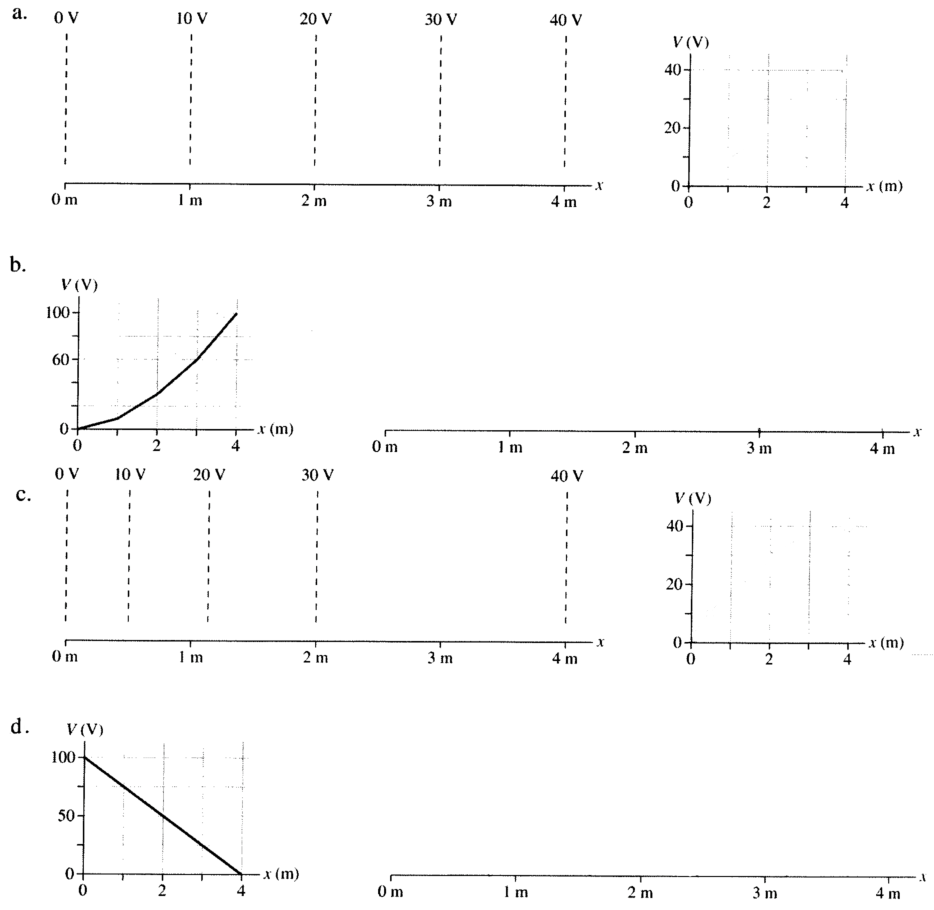
\includegraphics[scale=0.75]{A1}
	%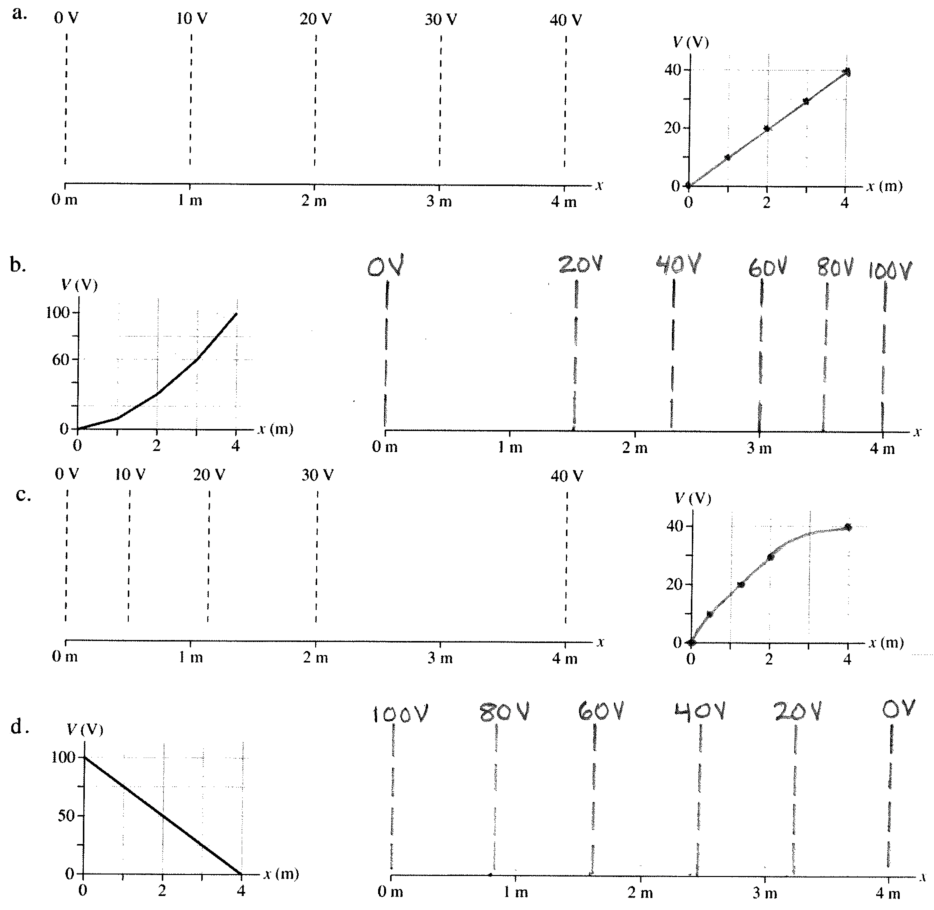
\includegraphics[scale=0.75]{A1Sol}%Solution
\end{center}

\pagebreak
\section*{Activity 2}%21
\excerpt{
An inflatable metal balloon of radius $ R $ is charged to a potential of 1000 V. After all wires and batteries are disconnected, the balloon is inflated to a new radius $ 2R $.
}
\excerpt{
(a) Does the potential of the balloon change as it is inflated? If so, by what factor? If not, why not?
}
% To reveal the solution, delete "\phantom{\parbox{\textwidth}{" from the beginning, and "}}" from the end.
\phantom{\parbox{\textwidth}{
Yes. The potential decreases by a factor of 2. Once the wires are disconnected, the charge $ Q $ on the balloon is constant. For a symmetric sphere of charge, Gauss' law tells us that the electric field outside is the same as that of a point charge $ Q $ at the center of the sphere. At the surface of the balloon at its initial radius, it has potential
\[
V_{1} = \frac{1}{4\pi\epsilon_{0}}\frac{Q}{R}.
\]
Once we inflate it, the new potential at the surface is
\[
V_{2} = \frac{1}{4\pi\epsilon_{0}}\frac{Q}{2R}.
\]
}}
\excerpt{
(b) Does the potential at a point at distance $ r = 4R $ change as the balloon is inflated? If so, by what factor? If not, why not?
}
% To reveal the solution, delete "\phantom{\parbox{\textwidth}{" from the beginning, and "}}" from the end.
\phantom{\parbox{\textwidth}{
No. As was remarked before, the potential outside of the sphere is the same as that of a point charge $ Q $ located at the center of the sphere. The distance $ r = 4R $ remains outside of the balloon as it is inflated, and $ Q $ is unchanged.
}}

\pagebreak
\section*{Activity 3}%22
\excerpt{
A small charged sphere of radius $ R_{1} $, mass $ m_{1} $, and positive charge $ q_{1} $ is shot head on with speed $ v_{1} $ from a long distance away toward a second small sphere having radius $ R_{2} $, mass $ m_{2} $, and positive charge $ q_{2} $. The second sphere is held in a fixed location and cannot move. The spheres repel each other, so sphere 1 will slow as it approaches sphere 2. If $ v_{1} $ is small, sphere 1 will reach a closest point, reverse direction, and be pushed away by sphere 2. If $ v_{1} $ is large, sphere 1 will crash into sphere 2. For what speed $ v_{1} $ does sphere 1 just barely touch sphere 2 as it reverses direction?
}
\excerpt{
(a) Begin by drawing a before and after pictorial representation. Initially, the spheres are far apart, and sphere 1 is heading toward sphere 2 with speed $ v_{1} $. The problem ends with the spheres touching. What is the speed of sphere 1 at this instant? How far apart are the centers of the spheres at this instant? Label the before and after pictures with complete information---all in symbolic form.
}
% To reveal the solution, delete "\phantom{\parbox{\textwidth}{" from the beginning, and "}}" from the end.
\phantom{\parbox{\textwidth}{
\begin{center}
	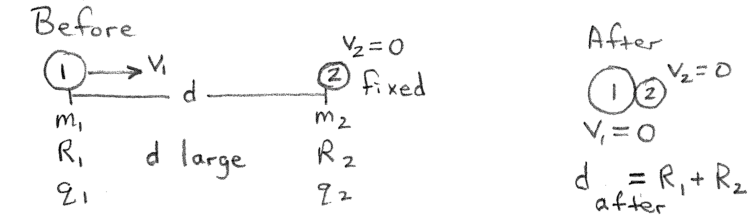
\includegraphics[scale=0.75]{A3a}
\end{center}
}}
\excerpt{
(b)We can treat this as an energy conservation problem, but first we have to identify the ``moving charge'' $ q $ and the ``source charge'' that creates the potential.
}
\begin{itemize}
	\item Which is the moving charge? %$ \qquad q_{1} $
	\item Which is the source charge? %$ \qquad q_{2} $
\end{itemize}
\excerpt{
(c) We're told the charges start ``a long distance away'' from each other. Based on that statement, what value can you assign to $ V_{i} $, the potential of the source charge at the initial position of the moving charge? Explain.
}
% To reveal the solution, delete "\phantom{\parbox{\textwidth}{" from the beginning, and "}}" from the end.
\phantom{\parbox{\textwidth}{
The initial potential $ V_{i} \approx 0 $ V, since $ V = \frac{1}{4\pi\epsilon_{0}}\frac{q_{2}}{d} $, and $ d $ is very large. \\
}}
\excerpt{
(d) Now write an expression in terms of the symbols defined above (and any constants that are needed) for the initial energy $ K_{i} + qV_{i} $.
}
% To reveal the solution, delete "\phantom{\parbox{\textwidth}{" from the beginning, and "}}" from the end.
\phantom{\parbox{\textwidth}{
\[
K_{i} + qV_{i} = \frac{1}{2}m_{1}v_{1}^{2} + 0
\]
}}
\excerpt{
(e) Referring to information on your visual overview, write an expression for the final energy.
}
% To reveal the solution, delete "\phantom{\parbox{\textwidth}{" from the beginning, and "}}" from the end.
\phantom{\parbox{\textwidth}{
\[
K_{f} + qV_{f} = 0 + \frac{1}{4\pi\epsilon_{0}}\frac{q_{1}q_{2}}{R_{1}+R_{2}}
\]
}}
\excerpt{
(f) Energy is conserved, so finish the problem by solving for $ v_{1} $.
}
% To reveal the solution, delete "\phantom{\parbox{\textwidth}{" from the beginning, and "}}" from the end.
\phantom{\parbox{\textwidth}{
Since energy is conserved,
\[
\frac{1}{2}m_{1}v_{1}^{2} = \frac{1}{4\pi\epsilon_{0}}\frac{q_{1}q_{2}}{R_{1}+R_{2}}.
\]
Rearranging, we find
\[
v_{1} = \left[\frac{q_{1}q_{2}}{2\pi\epsilon_{0}m_{1}(R_{1}+R_{2})}\right]^{1/2}.
\]
}}

\end{document}
